\chapter{Labotechnieken II: synthese en analyse in de praktijk}\label{ch:b2:lab-techniques-2}

Een grignardreactie mislukt op een maandagochtend: de kolf was gespoeld maar niet gedroogd, en de paar
druppels water die erin achterbleven, vernietigden het reagens terwijl het gevormd werd. Opnieuw uitgevoerd in glaswerk dat in een oven gedroogd is,
onder stikstof, met het halogenide druppel voor druppel toegevoegd aan een geroerde, gekoelde kolf, lukt
dezelfde reactie wel. De chemie veranderde niet; de opstelling wel. Dit hoofdstuk gaat over de praktijk die van een
reactie op papier een product in een flesje maakt: de reactie beheersen, lucht en water buitenhouden,
opwerken, zuiveren en bewijzen wat er gemaakt werd.

\begin{omfigure}
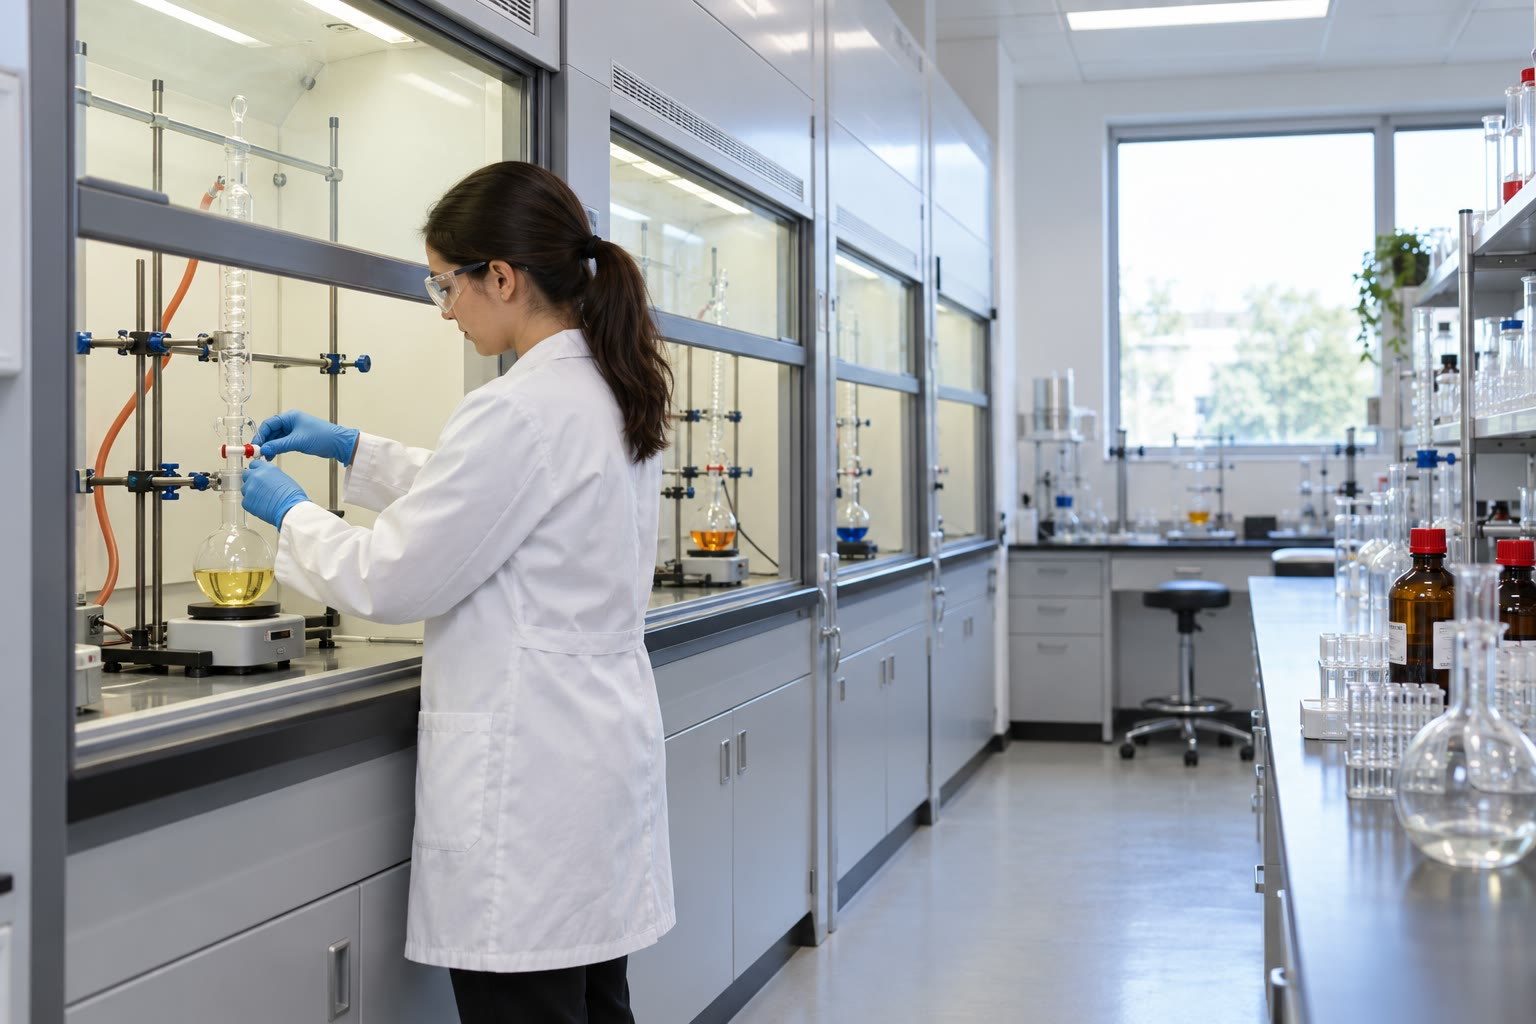
\includegraphics[width=0.56\linewidth]{images/book3/ai/b2-35-synthesis-lab.jpg}

{\small Een laboratorium voor organische synthese: reacties lopen in zuurkasten, kolven zijn op statieven geklemd
(illustratie).}
\end{omfigure}

\begin{recall}
Het deel van jaar~1: gevaren en GHS-etiketten, extractie, herkristallisatie, destillatie,
dunnelaagchromatografie en $R_f$, smeltpunt, grignardreagentia. \Cref{ch:b2:reaction-enthalpy}:
\omterm{def:b2:reaction-enthalpy:reaction-quantity}{reactie-enthalpie} en \omterm{def:b2:continuous-reactors:adiabatic-rise}{adiabatische temperatuurstijging}. \Cref{ch:b2:chromatography},
\cref{ch:b2:structure-determination} en \cref{ch:b2:measurement-statistics}: analyse.
\end{recall}

\section{Een reactie onder controle uitvoeren}

Een reactie in een kolf geeft haar warmte af waar ze plaatsvindt. De chemicus beheerst de temperatuur met een bad
(ijs en water, ijs en zout, droogijs en aceton voor de laagste temperaturen), met de terugvloeiing van een
kokend oplosmiddel, die de temperatuur begrenst tot het kookpunt terwijl de koeler de damp
terugstuurt, en met de snelheid waarmee een reagens toegevoegd wordt. Een inwendige thermometer, in de vloeistof en niet
in het bad, meet wat ertoe doet.

\begin{proposition}[Accumulatie]\label{prop:b2:lab-techniques-2:accumulation}
Als een reagens sneller toegevoegd wordt dan het reageert, hoopt de niet-gereageerde hoeveelheid $n_{\mathrm{acc}}$ zich op. Als
die dan in één keer reageert, zonder koeling, stijgt de temperatuur van het mengsel met warmtecapaciteit $C$ met
\begin{equation*}
\Delta T_{\mathrm{ad}} = \frac{n_{\mathrm{acc}}\,|\Delta_rH|}{C}.
\end{equation*}
\end{proposition}

\begin{proof}
De reactie van $n_{\mathrm{acc}}$ maakt bij constante druk $n_{\mathrm{acc}}|\Delta_rH|$ vrij
(\cref{ch:b2:reaction-enthalpy}); zonder warmte-uitwisseling verwarmt dat alles het mengsel, zoals bij de
\omterm{def:b2:reaction-enthalpy:flame-temperature}{adiabatische vlamtemperatuur} (\cref{def:b2:reaction-enthalpy:flame-temperature}): $C\Delta T =
n_{\mathrm{acc}}|\Delta_rH|$.
\end{proof}

Het gevaar is het grootst wanneer een reactie traag op gang komt, zoals grignardvormingen vaak doen: halogenide dat
vóór de initiatie toegevoegd wordt, stapelt zich op, en wanneer de reactie eindelijk start, gaat ze op hol. De regel is: voeg een kleine
portie toe, zie de reactie starten (opwarming, troebeling, zachte terugvloeiing), en voeg pas dan de rest toe in het
tempo dat de koeling kan volgen.

\section{Droge omstandigheden en inerte atmosfeer}

\begin{definition}[Inerte atmosfeer]\label{def:b2:lab-techniques-2:inert}
Een reactie wordt onder een \emph{inerte atmosfeer}\index{inerte atmosfeer} uitgevoerd wanneer de lucht in de opstelling
vervangen is door een niet-reactief gas, stikstof of argon, dat op een lichte overdruk gehouden wordt zodat er geen lucht
binnen kan.
\end{definition}

Organometaalreagentia, metaalhydriden en veel katalysatoren reageren met water en zuurstof. Glaswerk wordt
in een oven gedroogd en warm gemonteerd, of in een gasstroom uitgevlamd; oplosmiddelen worden droog gekocht of gedroogd
over een reagens dat met water reageert; vloeistoffen worden met spuiten via rubberen septa overgebracht.
Het gas vertrekt via een oliebubbelteller, die de stroom toont en verhindert dat lucht terugstroomt. De
schlenklijn en de handschoenkast, voor de gevoeligste verbindingen, komen in het deel van jaar~3.

\begin{omfigure}
\begin{tikzpicture}[lab/.style={font=\scriptsize, align=center}]
\fill[omDef!10] (-1.7,-0.3) rectangle (1.7,1.0);
\draw[om glass] (-1.7,1.2) -- (-1.7,-0.3) -- (1.7,-0.3) -- (1.7,1.2);
\foreach \x/\y in {-1.5/0.0,-1.45/0.55,1.3/0.05,1.3/0.6,-1.25/0.3,1.05/-0.15}{
  \draw[omDef!50, fill=white] (\x,\y) rectangle ++(0.18,0.18);}
\pic (f) at (0,0) {threeneck={0.35}{omThm!25}};
\pic[rotate=25] (d) at (f-l) {dropfunnel={0.5}{omMeth!20}};
\pic (c) at (f-c) {condenser};
\pic[rotate=-25] (t) at (0.0,0.42) {thermometer};
\pic (b) at (3.6,3.6) {bubbler};
\draw[thick, black!60] (0,6.25) -- (0,6.75) -- (3.25,6.75) -- (b-in);
\coordinate (dtop) at ($(f-l)+(-1.52,3.26)$);
\draw[thick, black!60] (dtop) -- ++(0,0.35) -- ++(-0.9,0) node[left, lab] {N$_2$};
\node[lab, anchor=north] at (0,-0.4) {ijsbad};
\node[lab, anchor=east] at (-1.9,2.6) {druppel-\\trechter};
\node[lab, anchor=west] at (0.55,5.0) {koeler};
\node[lab, anchor=west] at (1.75,2.6) {thermometer\\(inwendig)};
\node[lab, anchor=north] at (3.6,3.45) {bubbelteller (gasuitlaat)};
\end{tikzpicture}
\par\vspace{4pt}

{\small Een reactie onder stikstof (schematisch). Driehalskolf in een ijsbad, met een inwendige
thermometer in de vloeistof; het reagens wordt toegevoegd uit een drukvereffenende druppeltrechter waarlangs de
stikstof binnenkomt; het gas vertrekt via de koeler en een oliebubbelteller.}
\end{omfigure}

\begin{method}[Een droge reactie onder stikstof opstellen]\label{met:b2:lab-techniques-2:anhydrous}
\begin{enumerate}
  \item Droog het glaswerk in een oven en monteer het heet, met ingevette of omhulde slijpstukken; plaats een septum
        of de druppeltrechter, de koeler en de bubbelteller.
  \item Spoel met stikstof terwijl het afkoelt; houd de hele tijd een trage stroom aan (een bel om de één à twee seconden).
  \item Voeg vaste stoffen toe vóór het spoelen, droge oplosmiddelen en vloeibare reagentia met een spuit of canule via een
        septum.
  \item Koel of verwarm zoals gepland; begin de toevoeging met een kleine portie en controleer dat de reactie
        start voor je verdergaat.
\end{enumerate}
\end{method}

\section{Opwerking}

\begin{definition}[Opwerking]\label{def:b2:lab-techniques-2:work-up}
De \emph{opwerking}\index{opwerking} van een reactie is de reeks bewerkingen, na de reactie, die
het reactiemengsel omzet in het ruwe product: blussen, extraheren en wassen, drogen,
filtreren en het oplosmiddel afdampen.
\end{definition}

\begin{definition}[Zuur-base-extractie]\label{def:b2:lab-techniques-2:acid-base-extraction}
Een \emph{zuur-base-extractie}\index{zuur-base-extractie} scheidt zure, basische en neutrale organische
verbindingen die opgelost zijn in een organisch oplosmiddel, door de oplossing te wassen met waterige zuren of basen, die
één klasse verbindingen omzetten in ionen die naar het water overgaan.
\end{definition}

\begin{proposition}[Wie gaat waarheen]\label{prop:b2:lab-techniques-2:acid-base-extraction}
Waterig natriumwaterstofcarbonaat (pH 8.3) extraheert een carbonzuur ($\mathrm pK_a$ ongeveer 4) maar geen
fenol ($\mathrm pK_a$ ongeveer 10), dat natriumhydroxide vraagt; verdund zoutzuur extraheert een
amine waarvan het geconjugeerde zuur een $\mathrm pK_a$ van 4.6 of meer heeft; neutrale verbindingen blijven in de organische
laag.
% ledger: ph:NaHCO3, pka:benzoic, pka:phenol, pka:anilinium
\end{proposition}

\begin{proof}
Een deeltje is grotendeels in zijn basische vorm wanneer $\mathrm{pH} > \mathrm pK_a$, en voor meer dan 99~\% wanneer
$\mathrm{pH} > \mathrm pK_a + 2$. Bij pH 8.3 is benzoëzuur (4.2) voor meer dan 99~\% benzoaat, een ion
dat in het water blijft; fenol (9.99) is voor ongeveer 2~\% fenolaat ($10^{8.3 - 10.0}$) en blijft in wezen
in de organische laag, waarnaar de neutrale vorm zich verdeelt. In natriumhydroxide (pH boven 12) wordt fenol
omgezet in fenolaat. In verdund zoutzuur (pH ongeveer 1) is aniline (anilinium 4.6) voor meer dan
99~\% anilinium. Elk ion wordt, eenmaal in het water, teruggewonnen door de pH weer de andere kant op te brengen, wat
de neutrale verbinding terugvormt, en die daarna opnieuw te extraheren.
\end{proof}

\begin{omfigure}
\begin{tikzpicture}[x=1cm, y=1cm, st/.style={draw=black!70, rounded corners=2pt, fill=white,
  font=\scriptsize, align=center, inner sep=3pt, text width=3.0cm}, ar/.style={->, thick, black!70}]
\node[st, fill=omDef!10] (m) at (0,0) {benzoëzuur, fenol,\\aniline, naftaleen\\in ethoxyethaan};
\node[st, fill=omThm!10] (a1) at (5.0,0) {waterig: benzoaat\\$\to$ HCl $\to$ benzoëzuur};
\node[st] (o1) at (0,-1.6) {fenol, aniline,\\naftaleen};
\node[st, fill=omThm!10] (a2) at (5.0,-1.6) {waterig: fenolaat\\$\to$ HCl $\to$ fenol};
\node[st] (o2) at (0,-3.2) {aniline, naftaleen};
\node[st, fill=omThm!10] (a3) at (5.0,-3.2) {waterig: anilinium\\$\to$ NaOH $\to$ aniline};
\node[st, fill=omMeth!10] (o3) at (0,-4.8) {naftaleen\\(drogen, afdampen)};
\draw[ar] (m) -- node[above, font=\tiny] {wassen met NaHCO$_3$} (a1);
\draw[ar] (m) -- (o1); \draw[ar] (o1) -- node[above, font=\tiny] {wassen met NaOH} (a2);
\draw[ar] (o1) -- (o2); \draw[ar] (o2) -- node[above, font=\tiny] {wassen met HCl} (a3);
\draw[ar] (o2) -- (o3);
\pic at (8.6,-3.6) {sepfunnel={omDef!25}{omThm!20}};
\node[font=\scriptsize, align=center] at (8.6,-4.0) {scheitrechter};
\end{tikzpicture}
\par\vspace{4pt}

{\small Zuur-basescheiding van vier verbindingen (\cref{prop:b2:lab-techniques-2:acid-base-extraction}).
De organische laag (linkerkolom) verliest bij elke wasbeurt één klasse; elk waterig extract (rechts) geeft
zijn verbinding terug wanneer de pH omgekeerd wordt.}
\end{omfigure}

\begin{definition}[Droogmiddel]\label{def:b2:lab-techniques-2:drying-agent}
Een \emph{droogmiddel}\index{droogmiddel} is een watervrij zout, zoals magnesium- of natriumsulfaat,
dat het in een organische oplossing opgeloste water als hydratatiewater bindt en daarna door
filtratie verwijderd wordt.
\end{definition}

\begin{method}[Van de reactiekolf naar het ruwe product]\label{met:b2:lab-techniques-2:work-up}
\begin{enumerate}
  \item Blussen: vernietig de resterende reactieve reagentia met een geschikte waterige oplossing, langzaam en onder
        koeling.
  \item Extraheer naar een organisch oplosmiddel; scheid de lagen (controleer welke welke is door een druppel
        water toe te voegen); extraheer de waterlaag opnieuw.
  \item Was de samengevoegde organische lagen (zuur, base, dan pekel, een verzadigde natriumchlorideoplossing
        die het grootste deel van het opgeloste water verwijdert).
  \item Droog met een \omterm{def:b2:lab-techniques-2:drying-agent}{droogmiddel} tot een deel ervan vrij blijft bewegen; filtreer.
  \item Verwijder het oplosmiddel op een rotatieverdamper onder verlaagde druk; weeg het ruwe product.
\end{enumerate}
\end{method}

\section{Zuivering}

\begin{definition}[Flashchromatografie]\label{def:b2:lab-techniques-2:flash}
\emph{Flashchromatografie}\index{flashchromatografie} is preparatieve kolomchromatografie op silica waarbij
het elutiemiddel met een lichte gasdruk door de kolom geduwd wordt, zodat een scheiding van grammen
materiaal minuten duurt; het elutiemiddel wordt gekozen met dunnelaagchromatografie op dezelfde silica.
\end{definition}

\begin{proposition}[Kolomvolumes]\label{prop:b2:lab-techniques-2:column-volumes}
Een verbinding die op een dunnelaagplaat loopt bij $R_f$, verlaat een kolom met dezelfde silica en hetzelfde elutiemiddel na
ongeveer $1/R_f$ kolomvolumes elutiemiddel.
\end{proposition}

\begin{proof}[Redenering]
Op de plaat legt de verbinding $R_f$ keer de afstand van het oplosmiddelfront af: haar gemiddelde snelheid is $R_f$
keer die van het elutiemiddel. Op de kolom geeft dezelfde verdeling dezelfde verhouding van snelheden, dus de
verbinding heeft $1/R_f$ keer het volume elutiemiddel nodig dat de kolom vult (het dode volume) om eruit te
komen; in de taal van \cref{ch:b2:chromatography} is $R_f \approx 1/(1 + k)$. Een verbinding bij $R_f = 0.25$
komt eruit na ongeveer vier kolomvolumes, goed gescheiden van een verbinding bij 0.5 (twee volumes).
\end{proof}

\begin{omfigure}
\begin{tikzpicture}[lab/.style={font=\scriptsize, align=left, anchor=west}]
\pic (k) at (0,0) {chromcolumn={3.4}};
\node[lab] at (0.6,4.6) {elutiemiddel};
\node[lab] at (0.6,3.55) {zand};
\node[lab] at (0.6,2.2) {silicabed};
\foreach \i/\c in {0/white, 1/omThm!25, 2/omThm!25, 3/white, 4/omDef!25, 5/omDef!25, 6/white}{
  \pic at ({2.4+0.55*\i},-1.2) {testtube={0.45}{\c}};}
\node[font=\scriptsize] at (4.05,-1.6) {fracties 1 tot 7};
\pic at (7.6,-1.2) {tlcplate};
\foreach \j/\x in {2/7.15,3/7.45,5/7.75,6/8.05}{\node[font=\tiny] at (\x,-1.38) {\j};}
\fill[omThm] (7.45,0.95) circle (0.06); \fill[omThm] (7.15,0.95) circle (0.06);
\fill[omDef] (8.05,-0.05) circle (0.06); \fill[omDef] (7.75,-0.05) circle (0.06);
\node[font=\scriptsize, align=center] at (7.6,2.15) {DLC van de\\fracties};
\end{tikzpicture}
\par\vspace{4pt}

{\small \omterm{def:b2:lab-techniques-2:flash}{Flashchromatografie} (schematisch). Het ruwe product wordt boven op de silica aangebracht en geëlueerd;
het eluaat wordt in fracties opgevangen; een dunnelaagplaat van de fracties toont waar elke verbinding uitkwam
(hier de snelle, apolaire verbinding in fracties 2--3, de tragere in 5--6), en de zuivere fracties worden
samengevoegd.}
\end{omfigure}

\begin{method}[Een flashkolom uitvoeren]\label{met:b2:lab-techniques-2:flash}
\begin{enumerate}
  \item Kies het elutiemiddel met DLC: de gewenste verbinding bij een $R_f$ van ongeveer 0.25--0.35, zo ver mogelijk van
        de onzuiverheden.
  \item Pak de silica (ongeveer 30 tot 100 keer de massa van het ruwe product) als suspensie of droog; voeg een laag
        zand toe.
  \item Breng het ruwe product aan in zo weinig mogelijk oplosmiddel (of geadsorbeerd op een beetje silica).
  \item Elueer onder lichte druk; vang fracties op; controleer ze met DLC; voeg de zuivere samen en
        damp in.
\end{enumerate}
\end{method}

Vloeistoffen die rond hun kookpunt ontleden, worden gedestilleerd bij verlaagde druk, waar ze
lager koken.

\begin{definition}[Destillatie onder verlaagde druk]\label{def:b2:lab-techniques-2:reduced-pressure}
Een \emph{destillatie onder verlaagde druk}\index{destillatie onder verlaagde druk} wordt uitgevoerd
in een opstelling die via een manometer met een vacuümpomp verbonden is, bij een druk waarbij de vloeistof kookt op een
temperatuur die ze verdraagt.
\end{definition}

\begin{proposition}[Koken bij verlaagde druk]\label{prop:b2:lab-techniques-2:reduced-pressure}
Met $T_b$ de kooktemperatuur bij de referentiedruk $p^\circ$ en $\Delta_{\mathrm{vap}}H$
als constant beschouwd, wordt de kooktemperatuur bij druk $p$ gegeven door
\begin{equation*}
\frac{1}{T} = \frac{1}{T_b} - \frac{R}{\Delta_{\mathrm{vap}}H}\ln\frac{p}{p^\circ}.
\end{equation*}
\end{proposition}

\begin{proof}
Een vloeistof kookt wanneer haar dampdruk gelijk is aan de druk erboven. De relatie van Clausius--Clapeyron
uit de natuurkunde, $\mathrm d\ln p/\mathrm dT = \Delta_{\mathrm{vap}}H/(RT^2)$ voor een ideale damp en een
verwaarloosbaar vloeistofvolume, geeft na integratie tussen $(T_b, p^\circ)$ en $(T, p)$ $\ln(p/p^\circ) =
-(\Delta_{\mathrm{vap}}H/R)(1/T - 1/T_b)$; herschikken geeft het resultaat.
\end{proof}

\begin{omfigure}
\begin{tikzpicture}
\begin{axis}[width=0.72\linewidth, height=5.2cm, xmode=log, xmin=5, xmax=1100, ymin=0, ymax=190,
  xlabel={druk (\unit{mbar})}, ylabel={kooktemperatuur (\unit{\degreeCelsius})},
  label style={font=\small}, tick label style={font=\scriptsize}, grid=major, grid style={black!10},
  legend style={font=\scriptsize, at={(0.02,0.98)}, anchor=north west}, legend cell align=left]
\addplot[omDef, thick] table[x=p, y=bromobenzene] {figdata/out/bachelor-2-vacuum-boiling.dat};
\addplot[omThm, thick] table[x=p, y=benzaldehyde] {figdata/out/bachelor-2-vacuum-boiling.dat};
\addplot[only marks, mark=o, mark size=2pt, omDef] coordinates {(7,27.75)};
\addplot[only marks, mark=o, mark size=2pt, omThm] coordinates {(13,61.85)};
\legend{broombenzeen, benzaldehyde, gemeten}
\end{axis}
\end{tikzpicture}

{\small Kooktemperatuur tegen druk (\cref{prop:b2:lab-techniques-2:reduced-pressure}) met
de verdampingsenthalpieën en kookpunten uit het NIST WebBook. De cirkels zijn gemeten
kookpunten bij 7 en \qty{13}{mbar}, niet gebruikt voor de krommen: de eenvoudige vergelijking zit er hooguit enkele kelvin naast.
De druk verlagen van 1 bar tot \qty{20}{mbar} verlaagt de kookpunten met meer dan
\qty{100}{K}.}
% figdata: bachelor-2/vacuum-boiling.py
% ledger: tb:bromobenzene, dvap:bromobenzene, tbp:bromobenzene.7mbar, tb:benzaldehyde, dvap:benzaldehyde, tbp:benzaldehyde.13mbar
\end{omfigure}

\section{Zuiverheid en identiteit}

Een product wordt geïdentificeerd door zijn spectra en fysische constanten te vergelijken met die van de verwachte
verbinding (\cref{ch:b2:structure-determination}); zijn zuiverheid wordt afzonderlijk gemeten, omdat een product
de juiste verbinding kan zijn en toch nog enkele procenten van iets anders kan bevatten.

\begin{method}[Zuiverheid en rendement rapporteren]\label{met:b2:lab-techniques-2:purity}
\begin{enumerate}
  \item Controleer het smelttraject van een vaste stof (scherp en dicht bij de literatuurwaarde voor een zuivere
        verbinding) en zijn DLC (één vlek in twee elutiemiddelen).
  \item Meet de zuiverheid: oppervlakteprocent bij GC of HPLC (slechts een schatting tenzij de \omterm{def:b2:chromatography:quantitative}{responsfactoren} bekend zijn,
        \cref{ch:b2:chromatography}), of kwantitatieve proton-NMR, door een integraal van het product te vergelijken
        met een integraal van elke onzuiverheid, of met een afgewogen \omterm{def:b2:chromatography:quantitative}{interne standaard}.
  \item Reken om naar een massafractie $w$ product in het geïsoleerde materiaal.
  \item Rapporteer het rendement gecorrigeerd voor de zuiverheid: $\rho = w\,m/(n_{\mathrm{lim}}M)$, waarin $m$ de
        geïsoleerde massa is, $n_{\mathrm{lim}}$ de hoeveelheid beperkend reagens en $M$ de molaire massa.
\end{enumerate}
\end{method}

Bij een optisch actief product voegt de specifieke rotatie een controle van de stereochemische zuiverheid toe;
de enantiomere overmaat en haar meting worden behandeld in het deel van jaar~3.

\begin{safety}{\ghs[5mm]{GHS02}\,\ghs[5mm]{GHS06}\,\ghs[5mm]{GHS07}\,\ghs[5mm]{GHS08}\,\ghs[5mm]{GHS09}}
Ethoxyethaan en oxolaan zijn zeer licht ontvlambaar en vormen bij bewaring explosieve peroxiden; geen vlam in
het laboratorium, en test oude flessen voor je destilleert. Broombenzeen is ontvlambaar en giftig voor waterorganismen;
magnesiumkrullen zijn ontvlambaar. Vacuümglaswerk wordt gecontroleerd op stervormige barstjes en afgeschermd.
% ledger: ghs:ether, ghs:THF, ghs:bromobenzene, ghs:Mg, ghs:MgSO4
\end{safety}

\section{Oefeningen}

\begin{exercise}[$\star$]\label{exo:b2:lab-techniques-2:1}
Welk bad zou je gebruiken voor een reactie bij ongeveer \qty{0}{\degreeCelsius}, bij ongeveer
\qty{-15}{\degreeCelsius}, en bij \qty{-78}{\degreeCelsius}?
\end{exercise}

\begin{exercise}[$\star$]\label{exo:b2:lab-techniques-2:2}
Bij een extractie wordt dichloormethaan gebruikt, dat dichter is dan water. Welke laag is organisch? Hoe controleer je dat?
\end{exercise}

\begin{exercise}[$\star$]\label{exo:b2:lab-techniques-2:3}
Hoe weet je dat er genoeg magnesiumsulfaat aan een etheroplossing toegevoegd is?
\end{exercise}

\begin{exercise}[$\star$]\label{exo:b2:lab-techniques-2:4}
In hexaan--ethylacetaat 4\,:\,1 heeft een product $R_f = 0.65$ en een onzuiverheid 0.75. Wat zou je veranderen
voor een kolom, en in welke richting?
\end{exercise}

\begin{exercise}[$\star\star$]\label{exo:b2:lab-techniques-2:5}
Geef de volgorde van de wasbeurten die benzoëzuur, fenol, aniline en naftaleen scheiden uit een
etheroplossing, verantwoord elke stap met een $\mathrm pK_a$, en zeg hoe elke verbinding teruggewonnen wordt.
\end{exercise}

\begin{exercise}[$\star\star$]\label{exo:b2:lab-techniques-2:6}
Schat de kooktemperaturen van broombenzeen en benzaldehyde bij \qty{20}{mbar}.
\end{exercise}

\begin{exercise}[$\star\star$]\label{exo:b2:lab-techniques-2:7}
Tijdens een toevoeging heeft \qty{0.050}{mol} van een reagens zich niet-gereageerd opgestapeld. Met $\Delta_rH =
\qty{-200}{kJ/mol}$ en een warmtecapaciteit van \qty{400}{J/K} voor het mengsel (gegevens voor de oefening): welke
temperatuurstijging zou er kunnen volgen?
\end{exercise}

\begin{exercise}[$\star\star$]\label{exo:b2:lab-techniques-2:8}
Een HPLC-chromatogram toont het product bij 96.0~\% van de totale oppervlakte. Waarom is dat nog geen massazuiverheid? Een
protonspectrum van hetzelfde monster toont een singlet van het product (1H) met integraal 1.00 en een singlet van een onzuiverheid
(3H) met integraal 0.12; product \qty{200}{g/mol}, onzuiverheid \qty{100}{g/mol} (gegevens voor de oefening). Bereken de
massafractie product.
\end{exercise}

\begin{exercise}[$\star\star$]\label{exo:b2:lab-techniques-2:9}
Men verkrijgt \qty{4.10}{g} van een product (\qty{164}{g/mol}) met een zuiverheid van 95.0~\% (massa) uit \qty{0.0300}{mol}
beperkend reagens. Bereken het rendement, ongecorrigeerd en gecorrigeerd.
\end{exercise}

\begin{exercise}[$\star\star\star$]\label{exo:b2:lab-techniques-2:10}
Een grignardreactie gaf benzeen en bijna geen alcohol na toevoeging van het aldehyde. Som de
mogelijke oorzaken op en hoe je elk ervan vermijdt.
\end{exercise}

\begin{exercise}[$\star\star\star$]\label{exo:b2:lab-techniques-2:11}
Bij opschaling reageert \qty{1.00}{mol} van een halogenide met $\Delta_rH = \qty{-270}{kJ/mol}$ in een reactor waarvan de
koeling ten hoogste \qty{150}{W} afvoert (gegevens voor de oefening). Wat is de kortste veilige toevoegtijd? Wat
gebeurt er als de toevoeging sneller gaat?
\end{exercise}

\begin{exercise}[$\star\star\star$]\label{exo:b2:lab-techniques-2:12}
Een ruwe vaste stof van \qty{13.0}{g} zou gezuiverd kunnen worden door herkristallisatie (één stap, 80~\% terugwinning, zuiverheid
99~\%) of door \omterm{def:b2:lab-techniques-2:flash}{flashchromatografie} (95~\% terugwinning, zuiverheid 99.5~\%, \qty{1.5}{L} oplosmiddel) (gegevens voor de
oefening). Vergelijk de twee routes.
\end{exercise}

\section{Probleem: een grignardreactie zoals het hoort}

\begin{problem}[{Weekendprobleem --- gevaren en een droge opstelling, een beheerste toevoeging en het
accumulatiegevaar, de opwerking, zuivering door flashchromatografie en een voor de zuiverheid gecorrigeerd rendement}]
\label{pb:b2:lab-techniques-2:1}
Gegevens voor de oefening. Fenylmagnesiumbromide wordt gemaakt uit \qty{15.7}{g} broombenzeen en \qty{2.67}{g}
magnesiumkrullen in droog ethoxyethaan, daarna wordt \qty{9.55}{g} benzaldehyde toegevoegd; \omterm{def:b2:lab-techniques-2:work-up}{opwerking} met
waterig ammoniumchloride geeft difenylmethanol. Vorming van het reagens: $\Delta_rH =
\qty{-270}{kJ/mol}$; warmtecapaciteit van het mengsel \qty{170}{J/K}; start bij \qty{20}{\degreeCelsius}. DLC
(hexaan--ethylacetaat 9\,:\,1): bifenyl $R_f = 0.85$, difenylmethanol 0.25. Geïsoleerd na de kolom:
\qty{12.50}{g}. Proton-NMR van dit materiaal: het singlet van \ce{CH(OH)} (1H) integreert tot 1.00, het \omterm{def:b2:huckel:aromatic}{aromatische}
gebied tot 10.90. Molaire massa's (\unit{g/mol}): broombenzeen 157.01, benzaldehyde 106.12, difenylmethanol
184.24, bifenyl 154.21; Mg 24.305.
% ledger: ghs:ether, ghs:bromobenzene, ghs:Mg, ghs:benzaldehyde, ghs:NH4Cl, ghs:biphenyl, ghs:benzhydrol, tb:ether, aw:Mg, aw:C, aw:H, aw:Br, aw:O, nmr:biphenyl

\medskip
\noindent\textbf{Deel I --- Gevaren en opstelling.}
\begin{enumerate}
  \item Geef de belangrijkste gevaren van ethoxyethaan, broombenzeen en magnesium.
  \item Schrijf de reactie van fenylmagnesiumbromide met water op, en verklaar het in een oven gedroogde glaswerk.
  \item Waarom werken onder stikstof?
  \item Wat toont de bubbelteller, en wat verhindert hij?
  \item Waarom is ethoxyethaan hier een goed oplosmiddel?
  \item Bereken de hoeveelheden broombenzeen en magnesium. Welke is in overmaat?
\end{enumerate}

\medskip
\noindent\textbf{Deel II --- Beheerste toevoeging.}
\begin{enumerate}[resume]
  \item Welke warmte maakt de volledige vorming van het reagens vrij?
  \item Waarom wordt het broombenzeen druppel voor druppel toegevoegd?
  \item De reactie komt traag op gang, en 20~\% van het broombenzeen is toegevoegd voor dat gebeurt. Welke warmte
        kan er dan in één keer vrijkomen?
  \item Bereken de \omterm{def:b2:continuous-reactors:adiabatic-rise}{adiabatische temperatuurstijging}.
  \item Vergelijk de eindtemperatuur met het kookpunt van ethoxyethaan. Wat gebeurt er?
  \item Hoe moet de toevoeging uitgevoerd worden?
\end{enumerate}

\medskip
\noindent\textbf{Deel III --- Toevoeging en \omterm{def:b2:lab-techniques-2:work-up}{opwerking}.}
\begin{enumerate}[resume]
  \item Schrijf de reactie met benzaldehyde op en wijs het beperkende reagens aan.
  \item Waarom blussen met ammoniumchloride en niet met een sterk zuur?
  \item Welke laag is organisch in de scheitrechter?
  \item Waartoe dient het wassen met pekel?
  \item Hoe wordt de oplossing gedroogd, en hoe wordt het oplosmiddel verwijderd?
  \item Bifenyl is het belangrijkste bijproduct. Hoe ontstaat het, en wat begunstigt het?
\end{enumerate}

\medskip
\noindent\textbf{Deel IV --- Zuivering en zuiverheid.}
\begin{enumerate}[resume]
  \item Welke verbinding verlaat de kolom eerst?
  \item Na hoeveel kolomvolumes komt elke verbinding eruit?
  \item Bereken uit de NMR-integralen de molverhouding bifenyl/alcohol in het geïsoleerde
        materiaal.
  \item Bereken de massafractie difenylmethanol.
  \item Bereken de massa zuiver difenylmethanol.
  \item Bereken de theoretische massa.
  \item Bereken het rendement zonder correctie voor de zuiverheid.
  \item Geef het rendement gecorrigeerd voor de zuiverheid.
\end{enumerate}
\end{problem}
